\documentclass[11pt]{article}
\usepackage[margin=1in]{geometry}
\usepackage{amsmath,amssymb,amsthm,mathtools}
\usepackage{newtxtext,newtxmath}
\usepackage{graphicx,booktabs,microtype,enumitem,xcolor,fancyhdr}
\usepackage[colorlinks=true,linkcolor=blue!45!black,citecolor=blue!45!black,urlcolor=blue!45!black]{hyperref}
\usepackage[nameinlink,noabbrev]{cleveref}
\graphicspath{{../figures/}}
\hypersetup{pdftitle={Multiplication Presentations and Focal-Face Collapse in Algebraic Distance Certificates},pdfauthor={Shivam Gupta}}
\setlength{\parskip}{.3em}
\setlength{\parindent}{1.2em}
\setlist{itemsep=.15em,topsep=.3em}
\newtheorem{theorem}{Theorem}[section]
\newtheorem{proposition}[theorem]{Proposition}
\newtheorem{corollary}[theorem]{Corollary}
\newtheorem{lemma}[theorem]{Lemma}
\theoremstyle{definition}\newtheorem{definition}[theorem]{Definition}
\theoremstyle{remark}\newtheorem{remark}[theorem]{Remark}
\newcommand{\R}{\mathbb{R}}
\newcommand{\C}{\mathbb{C}}
\newcommand{\Sym}{\mathbb{S}}
\newcommand{\Vor}{\operatorname{Vor}}
\newcommand{\Span}{\operatorname{span}}
\newcommand{\diag}{\operatorname{diag}}
\newcommand{\vol}{\operatorname{vol}}
\newcommand{\norm}[1]{\left\lVert#1\right\rVert}
\pagestyle{fancy}\fancyhf{}\fancyhead[L]{\small Multiplication presentations and distance certificates}
\fancyhead[R]{\small Shivam Gupta}\fancyfoot[C]{\thepage}
\setlength{\headheight}{14pt}
\title{Multiplication Presentations and Focal-Face Collapse\\in Algebraic Distance Certificates}
\author{Shivam Gupta\\\small Independent Researcher, Delhi, India (corresponding author)\\\small\href{mailto:shivam1720406@gmail.com}{shivam1720406@gmail.com}}
\date{17 October 2026}
\begin{document}
\maketitle
\begin{abstract}
A polynomial reformulation preserves a feasible set but need not preserve its semidefinite distance certificates. We quantify this dependence for the affine moment curve $C_d=\{(t,t^2,\ldots,t^d):t\in\R\}$. Every choice of a factorization $k=i_k+j_k$ gives a smooth complete-intersection description with the same $d$ variables and $d-1$ quadratic equations. At the origin, the closed Voronoi cell has an exposed face of dimension $d-3$. We prove that the part certified by a chosen multiplication presentation has dimension exactly the number of factorizations avoiding the first coordinate. Thus all dimensions from zero to $d-3$ occur without changing problem size. A chain presentation collapses the face to a point; a balanced presentation preserves its dimension. We also prove a near-face volume-loss bound of order $\delta^{(d-3)/2}$, identify direction-dependent orders of boundary contact, and give an unbounded gap example in dimension four. Full quadratic closure restores exact certificates by classical univariate sum-of-squares theory; it is a reference formulation, not a new exactness theorem. Symbolic checks cover all 3,655 presentations in dimensions three through ten. An exact 315-point rational audit and 144 numerical semidefinite comparisons corroborate the analysis; the two sparse presentations are demonstrably incomparable away from the face. The results give a structural diagnostic for choosing multiplication equations in polynomial consistency and calibration models.
\end{abstract}
\noindent\textbf{Keywords:} algebraic distance optimization; Voronoi cells; semidefinite relaxation; quadratic reformulation; moment curve.\\
\noindent\textbf{MSC 2020:} 90C22, 14P10, 90C20.\\
\noindent\textbf{Code, data, and figures:} \url{https://github.com/shi1720/multiplication-presentations}.

\section{Introduction}
A solver may fail to certify the correct nearest point because of the equations supplied to it. This failure is distinct from an incorrect geometric model: two systems can generate the same ideal, have the same nonsingular real curve, and use the same number of quadratic equations, yet yield different convex Lagrangian certificates. Understanding this dependence is relevant when polynomial constraints are assembled from an expression graph, as in monomial-feature consistency, scalar calibration, and polynomial model compilation.

The general phenomenon is established. Cifuentes, Harris, and Sturmfels describe the geometry of semidefinite exactness and exhibit its dependence on the defining equations \cite{chs}. Lindberg and Rodriguez study invariance under changes of generators \cite{lr}. In particular, the twisted cubic and its strengthening by an implied quadric are already known examples \cite[Examples 6.1--6.2]{chs}. Our question is more specific: \emph{how much of an intrinsic Voronoi face can be lost solely through the choice of multiplication factors, at fixed formulation size?}

We answer this question for $C_d$, the affine moment curve. For every $k=2,\ldots,d$, choose $1\le i_k\le j_k<k$ with $i_k+j_k=k$, and impose
\begin{equation}\label{eq:presentation}
 f_k(x)=x_{i_k}x_{j_k}-x_k=0.
\end{equation}
All such systems generate the same ideal. Their Jacobian at zero has rank $d-1$. A chain uses $x_k=x_1x_{k-1}$; a balanced system uses $x_k=x_{\lfloor k/2\rfloor}x_{\lceil k/2\rceil}$. Both descriptions have precisely $d-1$ equations.

At the origin, write a normal data point as $u=(0,u_2,\ldots,u_d)$. The supporting hyperplane $u_2=1/2$ meets the closed Voronoi cell in a face $F_d$ of dimension $d-3$. The main theorem classifies the dimension of its certified portion for every system \eqref{eq:presentation}. Whenever a chosen product uses $x_1$, positive semidefiniteness forces its associated normal coordinate to vanish on this face. Products avoiding $x_1$ remain free in a relative neighborhood. This simple condition accounts for an arbitrarily large dimensional loss as $d$ increases.

The loss is not confined to boundary points. At $u_2=1/2-\delta$, a balanced presentation certifies a prism with a fixed-width $(d-3)$-dimensional section, while the chain restricts all higher normal coordinates to a ball of radius $\sqrt{2\delta}$. The fraction certified by the chain in that prism is at most a constant times $\delta^{(d-3)/2}$. In dimension four, the true face contains an unbounded ray that the balanced formulation certifies exactly, while the chain's vertical boundary gap grows quadratically.

The contributions are the dimension classification, its enumerator over all multiplication presentations, the near-face volume estimate, and the explicit contact and unbounded-gap calculations. Complete quadratic closure and its exactness on the moment curve are established foundations, included to provide an exact reference and clarify the cost of repairing a formulation. The computational study verifies these statements through separate algebraic, real-root, and semidefinite routes. We do not propose a universally superior sparse formulation or infer industrial performance from synthetic instances.

\section{Context and prior results}\label{sec:related}
\paragraph{Algebraic nearest-point geometry.}
The Euclidean distance degree counts complex critical points of a generic squared-distance problem and provides an algebraic perspective on projection \cite{eddegree}. Voronoi cells instead fix a point on the variety and collect ambient data for which it is a nearest point. Cifuentes, Ranestad, Sturmfels, and Weinstein develop their algebraic boundaries and spectrahedral inner approximations \cite{voronoi}. Their Problem 4.4 asks about tangency between these boundaries. Our contact calculation addresses a restricted family at a distinguished point; it does not resolve that general problem.

\paragraph{Dependence on generators.}
The master-spectrahedron construction in \cite{chs,voronoi} supplies the certificate used below. The known cubic example already has a parabolic inner boundary and a quartic true boundary. Lindberg and Rodriguez show that generator invariance holds under suitable hypotheses, including a complete-intersection condition on the highest homogeneous parts \cite[Theorem 2.4]{lr}. Our chain systems do not satisfy that condition: their quadratic parts have the common factor $x_1$, and their common zero set has dimension $d-1$, rather than the expected one. The affine systems themselves remain smooth complete intersections. We quantify the resulting failure for every recursive factorization, rather than claim generator dependence as a new observation.

\paragraph{Quadratic reformulation.}
Reformulating a polynomial program through monomial substitutions is a standard optimization technique. Mevissen and Kojima compare transformation heuristics and the quality of the resulting SDP relaxations \cite{mk}. Karia, Adjiman, and Chachuat investigate quadratic reformulation and redundant constraints in global mixed-integer polynomial optimization \cite{kac}. Our invariant is the dimension of a certified exposed face, not the number of added variables or a branch-and-bound runtime. It separates formulations with identical variable and equation counts.

\paragraph{Complete quadratic closure.}
Nonnegative univariate polynomials are sums of squares. More generally, nonnegative quadratic forms on totally real varieties of minimal degree are sums of squares of linear forms \cite{bsv}. This includes the projective rational normal curve and explains exactness after using the full quadratic relation space, as already noted in \cite[Remark 6.3]{chs}. We use that consequence as a baseline. General geometric descriptions of higher-order exactness cones appear in \cite{henrion}. None of these general exactness results, by themselves, specifies which face dimensions are retained by the restricted systems \eqref{eq:presentation}.

\begin{table}[t]
\centering\small
\begin{tabular}{p{.23\linewidth}p{.32\linewidth}p{.35\linewidth}}
\toprule
Established result & Role here & Specific question studied here\\\midrule
Master spectrahedron \cite{chs} & Convex Lagrangian certificate & Which factor choices force face coordinates to zero?\\
Generator invariance \cite{lr} & Conditions preventing dependence & Exact dimension loss outside those conditions\\
Cubic examples \cite{chs,voronoi} & Known low-dimensional precedent & Classification and volume loss for arbitrary $d$\\
Minimal-degree SOS \cite{bsv} & Exact full-closure reference & Sparse loss before completion\\
Quadratic reformulation \cite{mk,kac} & Computational setting & Geometry at fixed variable/equation counts\\\bottomrule
\end{tabular}
\caption{Contribution boundary. The present work quantifies a restricted structural effect; it does not introduce presentation dependence or moment-curve exactness.}\label{tab:prior}
\end{table}

\section{Geometry and the certificate matrix}\label{sec:setup}
Fix $d\ge3$ and let $\gamma_d(t)=(t,t^2,\ldots,t^d)$. We use the \emph{closed} Voronoi cell
\begin{equation}\label{eq:vor}
 V_d=\Vor_{C_d}(0)=\{u\in\R^d:\norm{\gamma_d(t)-u}^2\ge\norm{u}^2\ \text{for all }t\in\R\}.
\end{equation}
Ties are allowed. Membership asserts global optimality of zero, not uniqueness or a positive-definite certificate. Since $\gamma'_d(0)=e_1$, first-order optimality requires $u_1=0$. For such $u$,
\begin{align}
 D_u(t)&=\norm{\gamma_d(t)-u}^2-\norm{u}^2=t^2R_u(t),\label{eq:D}\\
 R_u(t)&=\sum_{j=1}^d t^{2j-2}-2\sum_{k=2}^d u_kt^{k-2}.\label{eq:R}
\end{align}
Continuity at $t=0$ gives the exact membership criterion $u\in V_d$ if and only if $R_u\ge0$ on $\R$. The term $R_u(0)=1-2u_2$ proves $u_2\le1/2$.

\begin{definition}
A multiplication presentation $P$ is a tuple $((i_k,j_k))_{k=2}^d$ satisfying \eqref{eq:presentation}. Its certificate set $S_P$ consists of the normal data $u$ admitting a convex quadratic Lagrangian whose minimum occurs at zero for the distance objective and the equations $f_k=0$.
\end{definition}

Let $A_{ii}=e_ie_i^T$, and for $i<j$ let $A_{ij}=(e_ie_j^T+e_je_i^T)/2$. Thus $x^TA_{ij}x=x_ix_j$.

\begin{lemma}\label{lem:matrix}
Every multiplication presentation generates $I(C_d)$ and defines a smooth complete intersection. Its certificate set is
\begin{equation}\label{eq:H}
 S_P=\{u:u_1=0,\ H_P(u):=I_d-2\sum_{k=2}^d u_k A_{i_kj_k}\succeq0\}\subseteq V_d.
\end{equation}
The multipliers in this centered certificate are unique.
\end{lemma}
\begin{proof}
Inductively, $x_k=x_{i_k}x_{j_k}=x_1^k$ in the quotient by $(f_2,\ldots,f_d)$. More explicitly, $x_k-x_1^k$ lies in this ideal by substituting the relations for the two lower-index factors. Conversely each $f_k$ vanishes under $x_j=t^j$. The quotient is therefore $\R[x_1]$ and its kernel is $I(C_d)$. In the Jacobian, the submatrix with columns $x_2,\ldots,x_d$ is lower triangular with diagonal $-1$, at every point. Its rank is $d-1$.

Write the centered ambient objective as $q_u(x)=x^Tx-2u^Tx$. In $L=q_u-\sum_{k=2}^d\lambda_k f_k$, stationarity at zero forces $-2u_k+\lambda_k=0$. Hence $\lambda_k=2u_k$, and $L(x)=x^TH_P(u)x$. Convexity is exactly $H_P(u)\succeq0$. On the curve $L=q_u=D_u$, so nonnegativity of this quadratic form proves membership in $V_d$. Conversely any convex stationary Lagrangian has the same multipliers and matrix.
\end{proof}

The matrix in \eqref{eq:H} has order $d$. The usual homogenized Shor primal matrix has order $d+1$; the centered dual certificate eliminates its constant row and column. Comparisons below keep both conventions fixed across presentations.

\section{A complete classification on the exposed face}\label{sec:main}
Define
\begin{equation}
 F_d=V_d\cap\{u_2=1/2\},\qquad
 B(P)=\{k\in\{3,\ldots,d\}:i_k=1\},\qquad
 a(P)=\#\{k\ge3:i_k>1\}.
\end{equation}
The term \emph{focal face} refers here to this explicitly defined exposed face: $D''_u(0)=0$ on its supporting hyperplane. No identification with an entire medial axis is intended.

\begin{theorem}[Face dimension determined by multiplication factors]\label{thm:face}
For every $d\ge3$:
\begin{enumerate}
\item The face $F_d$ has affine hull $\{u_1=0,u_2=1/2,u_3=0\}$ and dimension $d-3$. In that affine space it is described by
\begin{equation}\label{eq:facepoly}
 \sum_{j=2}^d t^{2j-4}-2\sum_{k=4}^d u_kt^{k-4}\ge0\quad\text{for every }t\in\R.
\end{equation}
\item For every multiplication presentation,
\begin{equation}\label{eq:forced}
 S_P\cap F_d\ \subseteq\ \{u_k=0:k\in B(P)\},\qquad
 \dim(S_P\cap F_d)=a(P).
\end{equation}
\item The chain presentation has $S_P\cap F_d=\{(0,1/2,0,\ldots,0)\}$. The balanced presentation has $\dim(S_P\cap F_d)=d-3$. Every intermediate dimension occurs at identical variable, equation, and matrix counts.
\end{enumerate}
\end{theorem}
\begin{proof}
At $u_2=1/2$, \eqref{eq:R} starts with $-2u_3t+O(t^2)$. Nonnegativity for both signs of $t$ forces $u_3=0$. Factoring the remaining $t^2$ from $R_u$ gives \eqref{eq:facepoly}. At zero tail this polynomial is $1+t^2+\cdots+t^{2d-4}$.

Let $L=\sum_{k=4}^d|u_k|$. For every exponent $0\le p\le d-4$, $|t|^p\le1+|t|^{2d-4}$. Thus for $L<1/2$ the polynomial in \eqref{eq:facepoly} is strictly positive, because its first and last terms alone dominate $2L(1+|t|^{2d-4})$. For $d=3$ the tail is empty and the assertion follows directly. This proves that $F_d$ contains a relative neighborhood of zero tail, establishing its affine hull and dimension.

In every presentation the $k=2$ split is $(1,1)$, so on the supporting hyperplane $H_{11}=0$. A positive semidefinite matrix with a zero diagonal entry has an identically zero corresponding row: each $2\times2$ principal minor gives $-|H_{1j}|^2\ge0$. For $k\ge3$ with $i_k=1$, the entry $H_{1,k-1}=-u_k$. No other split contributes to that entry, since the coordinate sum determines $k$. Therefore every coordinate in $B(P)$ is forced to zero.

Conversely set these forced coordinates to zero. The first row and column then vanish, while the remaining block is the identity at zero tail. For sufficiently small free coordinates it is positive definite. This provides an $a(P)$-dimensional relative neighborhood in $S_P\cap F_d$. The forced coordinates give the matching upper bound on dimension.

The chain uses $i_k=1$ for every $k$. A balanced split uses $i_3=1$ and $i_k\ge2$ for every $k\ge4$. At each $k\ge4$ one may independently choose either $(1,k-1)$ or a split avoiding one. Hence all dimensions $0,\ldots,d-3$ occur.
\end{proof}

\begin{corollary}[Enumerator]\label{cor:enumerator}
Counting unordered factor pairs $i_k\le j_k$, the number of presentations with certified face dimension $a$ is the coefficient of $z^a$ in
\begin{equation}\label{eq:enumerator}
 E_d(z)=\prod_{k=3}^d\left(1+(\lfloor k/2\rfloor-1)z\right).
\end{equation}
In particular, there are $\prod_{k=2}^d\lfloor k/2\rfloor$ presentations.
\end{corollary}
\begin{proof}
For coordinate $k$ exactly one split uses factor one, and $\lfloor k/2\rfloor-1$ avoid it. Choices at different coordinates are independent. Multiply their dimension-generating factors.
\end{proof}

The classification is stronger than comparing two defining sets after adding a redundant equation. It identifies all possible face dimensions while keeping exactly one quadratic equation per nontrivial power. The number of factors alone cannot detect the failure.

\begin{corollary}[Positive diagonal metrics]\label{cor:weighted}
Replace the objective by $\sum_{k=1}^d b_k(x_k-u_k)^2$, where all $b_k>0$. The supporting value becomes $u_2=b_1/(2b_2)$. The true exposed face still has dimension $d-3$, and every presentation retains exactly $a(P)$ dimensions on it.
\end{corollary}
\begin{proof}
The certificate is $\diag(b)-2\sum_{k=2}^d b_ku_kA_{i_kj_k}$. At the supporting value its $(1,1)$ entry is zero, and the same principal-minor argument forces $u_k=0$ for $k\in B(P)$. The remaining positive diagonal block remains positive definite for small free coordinates. In the true distance polynomial the linear coefficient after the first factorization is $-2b_3u_3$, so $u_3=0$. The counterpart of \eqref{eq:facepoly} is $\sum_{j=2}^d b_jt^{2j-4}-2\sum_{k=4}^d b_ku_kt^{k-4}$. Its constant and leading terms dominate small tail perturbations, exactly as above.
\end{proof}

\section{Loss near the face and orders of contact}\label{sec:contact}
\subsection{A volume bound at positive distance from the supporting hyperplane}
For the chain, the Schur complement in \eqref{eq:H} gives the complete formula
\begin{equation}\label{eq:chain}
 S_{\rm ch}=\left\{u:u_1=0,\quad 2u_2+\sum_{k=3}^d u_k^2\le1\right\}.
\end{equation}
All coordinates with index at least two have unit diagonal except for $H_{11}=1-2u_2$; the off-diagonal first row contains $-u_3,\ldots,-u_d$ and a final zero.

For $d\ge4$ put $n=d-3$, write $u=(0,1/2-\delta,w,z)$ with $z\in\R^n$, and fix $0<r<1/2$. Consider the $(d-2)$-dimensional normal-slice prism
\begin{equation}\label{eq:prism}
 K_{\delta,r}=\{(w,z):\norm{z}_1\le r,\quad |w|\le\sqrt{2\delta(1-2r)}\},\qquad\delta>0.
\end{equation}

\begin{theorem}[Near-face volume loss]\label{thm:volume}
The balanced presentation certifies every point of $K_{\delta,r}$. Let $\kappa_m=\pi^{m/2}/\Gamma(m/2+1)$ be the volume of the Euclidean unit ball in $\R^m$. The fraction of $K_{\delta,r}$ certified by the chain is bounded above by
\begin{equation}\label{eq:volume}
 \min\left\{1,\ \frac{\kappa_{n+1}(2\delta)^{n/2}n!}
 {2^{n+1}r^n\sqrt{1-2r}}\right\}.
\end{equation}
For fixed $d$ and $r$, this fraction tends to zero at least as fast as $\delta^{(d-3)/2}$.
\end{theorem}
\begin{proof}
In the balanced presentation the first coordinate participates only in the equations for $k=2,3$. Its matrix has block form
\[
 H_{\rm bal}=\begin{pmatrix}2\delta&-we_1^T\\-we_1&B(z)\end{pmatrix},\qquad
 B(z)=I_{d-1}-2\sum_{k=4}^d u_k\widetilde A_{i_kj_k}.
\]
Each $\widetilde A$ has operator norm at most one, so $B(z)\succeq(1-2r)I$. The Schur complement is nonnegative whenever $w^2\le2\delta(1-2r)$, proving the first claim.

The chain certifies the Euclidean ball $w^2+\norm{z}_2^2\le2\delta$, of volume $\kappa_{n+1}(2\delta)^{(n+1)/2}$. The prism has volume $2\sqrt{2\delta(1-2r)}\,2^nr^n/n!$. Bound the intersection by the volume of the ball and divide. The trivial upper bound one completes \eqref{eq:volume}.
\end{proof}

This is a statement about Lebesgue measure on each fixed-$u_2$ normal slice, not a distribution-free failure probability. For every $\delta>0$, the prism has nonempty relative interior. Thus the effect extends beyond a measure-zero face. The exponent is an upper-bound rate; the theorem does not assert an asymptotic equality for the intersection volume.

\subsection{Fourth-order contact in the cubic normal direction}
Set $u_3=w$ and $u_4=\cdots=u_d=0$. Let $b_d(w)$ denote the largest feasible $u_2$ in the true cell. With
\begin{equation}
 G_d(s)=\sum_{r=1}^{d-1}s^{2r},
\end{equation}
we have $b_d(w)=(1+\min_s(G_d(s)-2ws))/2$. Since $G_d''>0$, the minimizer is unique.

\begin{proposition}\label{prop:contact}
The true slice boundary has the parameterization
\begin{equation}\label{eq:parameter}
 w=\sum_{r=1}^{d-1}r s^{2r-1},\qquad
 b_d(w)=\frac12\left(1-\sum_{r=1}^{d-1}(2r-1)s^{2r}\right).
\end{equation}
For every $d\ge3$, as $w\to0$,
\begin{equation}\label{eq:contact}
 b_d(w)=\frac12-\frac12w^2+\frac12w^4+O(w^6).
\end{equation}
Consequently its vertical gap above the chain boundary is $w^4/2+O(w^6)$. As $|w|\to\infty$,
\begin{equation}\label{eq:asymptotic}
 b_d(w)\sim-\frac{2d-3}{2}(d-1)^{-\frac{2d-2}{2d-3}}
 |w|^{\frac{2d-2}{2d-3}}.
\end{equation}
\end{proposition}
\begin{proof}
The derivative equation is $G'_d(s)=2w$. Substitution into the minimum gives \eqref{eq:parameter}. Near zero, $w=s+2s^3+O(s^5)$, hence $s=w-2w^3+O(w^5)$. Substituting into $b_d=(1-s^2-3s^4+O(s^6))/2$ gives \eqref{eq:contact}. At infinity, the highest term yields $s\sim\operatorname{sgn}(w)(|w|/(d-1))^{1/(2d-3)}$; substituting the highest term of $b_d$ proves \eqref{eq:asymptotic}.
\end{proof}

For $d=3$, the baseline curves are the published twisted-cubic example \cite{chs,voronoi}. The expansion makes the contact order explicit; the family calculation extends it to all $d$. For $d\ge4$ contact is anisotropic: along $u_3=0$ and sufficiently small nonzero $(u_4,\ldots,u_d)=z$, the true boundary stays exactly $u_2=1/2$, while the chain boundary is $1/2-\norm{z}_2^2/2$. The vertical gap is quadratic in these directions. Fourth-order contact along one slice therefore does not imply fourth-order contact in the full normal space.

\begin{figure}[t]
\centering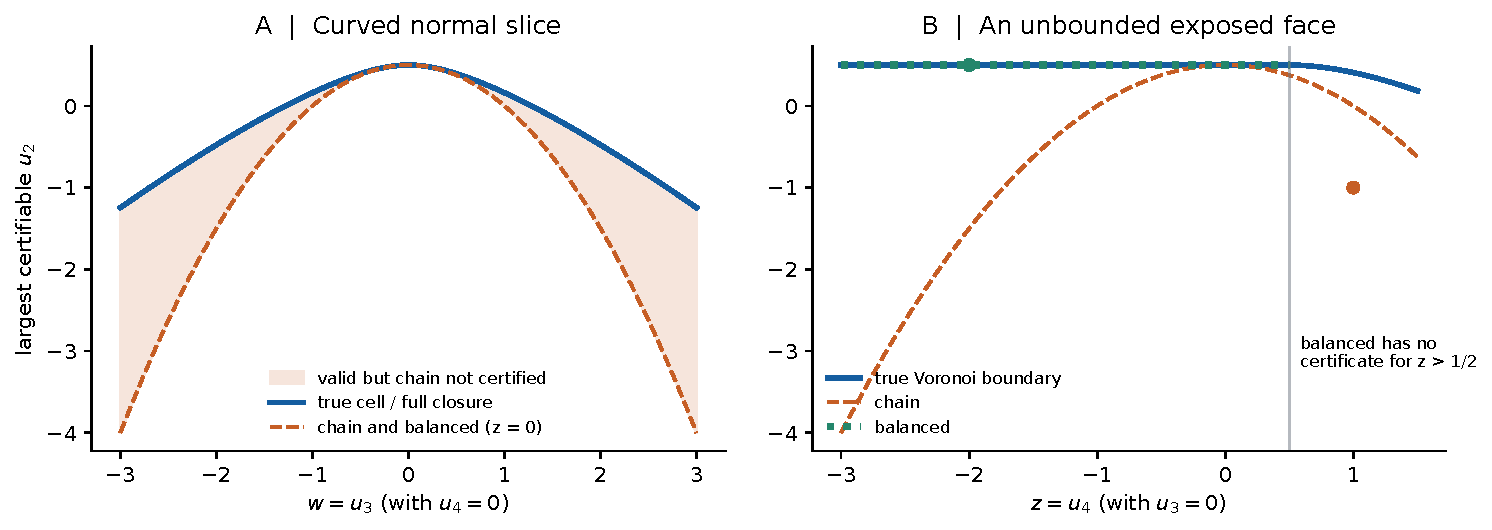
\includegraphics[width=\linewidth]{normal_slices.pdf}
\caption{Two normal slices for $C_4$. A: the exact boundary in the $u_3$ direction lies above the identical chain and balanced slice boundaries at $u_4=0$. B: at $u_3=0$, the balanced formulation preserves the complete exposed ray $u_2=1/2$, $u_4\le1/2$; the chain misses every nonzero point on it. The balanced formulation has no certificate when $u_4>1/2$, even though some such data belong to the true cell. Curves use scalar polynomial calculations, not sampled solver success rates.}\label{fig:slices}
\end{figure}

\begin{figure}[t]
\centering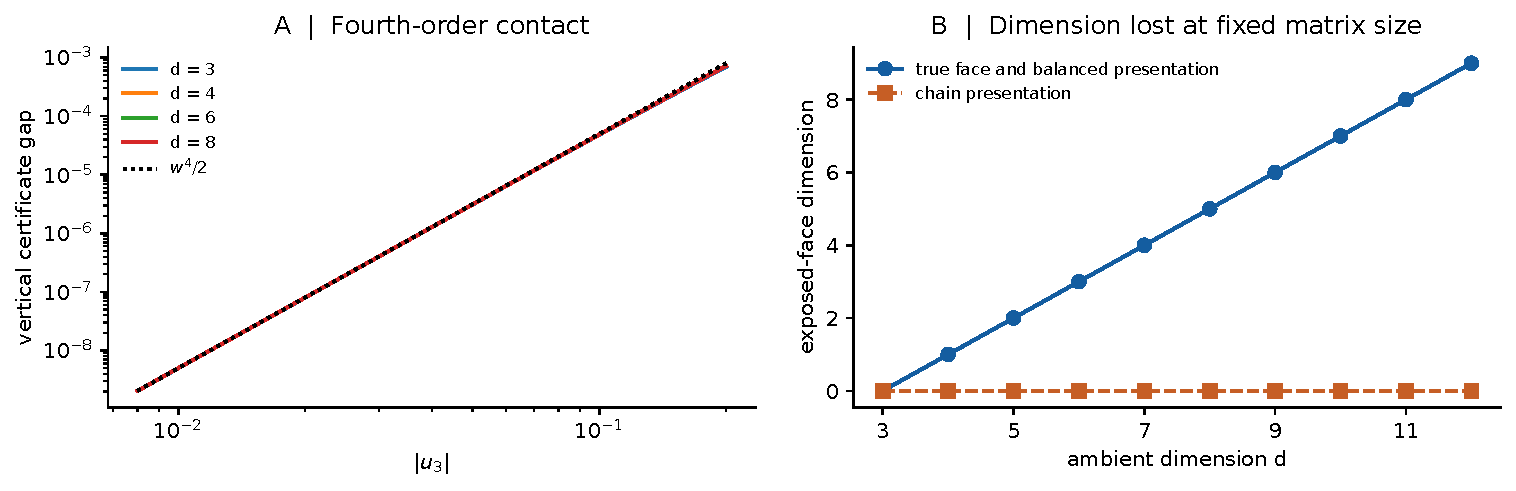
\includegraphics[width=\linewidth]{contact_and_dimension.pdf}
\caption{Boundary contact and face dimensions. A: the gap approaches $w^4/2$ for all displayed dimensions. B: the true exposed-face dimension and balanced certified-face dimension are $d-3$, while the chain retains zero dimensions. The lines display proved formulas.}\label{fig:contact}
\end{figure}

\section{Dimension four: an unbounded gap and incomparable formulations}\label{sec:quartic}
The two presentations of $C_4$ are
\begin{align*}
 P_{\rm ch}:&\quad x_2=x_1^2,\quad x_3=x_1x_2,\quad x_4=x_1x_3,\\
 P_{\rm bal}:&\quad x_2=x_1^2,\quad x_3=x_1x_2,\quad x_4=x_2^2.
\end{align*}
For $u=(0,v,w,z)$ their matrices are
\begin{equation}\label{eq:fourmatrices}
 H_{\rm ch}=\begin{pmatrix}1-2v&-w&-z&0\\-w&1&0&0\\-z&0&1&0\\0&0&0&1\end{pmatrix},\qquad
 H_{\rm bal}=\begin{pmatrix}1-2v&-w&0&0\\-w&1-2z&0&0\\0&0&1&0\\0&0&0&1\end{pmatrix}.
\end{equation}
Thus the chain requires $2v+w^2+z^2\le1$. The balanced system requires
\begin{equation}\label{eq:balanced4}
 1-2v\ge0,\quad 1-2z\ge0,\quad (1-2v)(1-2z)\ge w^2.
\end{equation}
These inequalities include singular edge cases; division by $1-2z$ would omit them.

At $v=1/2$, the exact criterion \eqref{eq:facepoly} becomes
\[
 w=0,\qquad 1-2z+t^2+t^4\ge0\quad\text{for all }t.
\]
Therefore $F_4=\{(0,1/2,0,z):z\le1/2\}$. The balanced system certifies the entire face, while the chain certifies only $z=0$. Along $w=0$ and $z\le1/2$, the true largest value of $v$ is $1/2$; the chain's largest value is $(1-z^2)/2$. Its vertical loss is exactly $z^2/2$, unbounded as $z\to-\infty$. All these face points have zero as their unique nearest point: $D_u(t)=t^4(1-2z+t^2+t^4)>0$ for $t\ne0$.

The balanced system does not dominate the chain. At $(0,-1,0,1)$, $H_{\rm ch}\succ0$ but $H_{\rm bal}$ has a negative diagonal entry. At $(0,1/2,0,-2)$, the balanced certificate is positive semidefinite and the chain fails. By \cref{lem:matrix}, both points are in $V_4$. The first counterexample also remains valid under small perturbations, so incomparability is not solely a boundary effect. Combining certificates from multiple presentations can improve coverage, but choosing the balanced system universally is not justified by \cref{thm:face}.

\section{Full quadratic closure as an exact reference}\label{sec:closure}
Let $x_0=1$. Restriction of an ambient quadratic to $C_d$ sends $x_ix_j$ to $t^{i+j}$, for $0\le i\le j\le d$. Its kernel $I_2(C_d)=I(C_d)\cap\R[x]_{\le2}$ consists of linear combinations of collisions
\begin{equation}\label{eq:collisions}
 x_ix_j-x_kx_\ell,\qquad i+j=k+\ell.
\end{equation}
Every power $t^s$, $0\le s\le2d$, occurs, so restriction is surjective and
\begin{equation}\label{eq:count}
 \dim I_2(C_d)=\binom{d+2}{2}-(2d+1)=\frac{d(d-1)}2.
\end{equation}
Use a basis of this vector space, rather than only one recursive product per coordinate.

\begin{proposition}[Classical exactness, specialized]\label{prop:closure}
For every $u\in V_d$, there is a matrix $H\succeq0$ such that
\begin{equation}\label{eq:gram}
 D_u(t)=\gamma_d(t)^TH\gamma_d(t).
\end{equation}
The difference $q_u(x)-x^THx$ belongs to $I_2(C_d)$. Hence full quadratic closure certifies the entire closed cell $V_d$ using a centered matrix of order $d$.
\end{proposition}
\begin{proof}
The nonnegative univariate polynomial $D_u$ has degree $2d$ and vanishes at zero. By the univariate sum-of-squares theorem it is a sum $\sum_r p_r(t)^2$ with $\deg p_r\le d$. Evaluating at zero forces each $p_r(0)=0$, so each $p_r$ is a linear combination of $t,\ldots,t^d$. The sum of the outer products of its coefficient vectors gives $H\succeq0$. Restricting $q_u-x^THx$ to the curve gives zero, which proves its membership in the quadratic kernel.
\end{proof}

This proposition is an elementary instance of the established minimal-degree result \cite{bsv,chs}. It is included for completeness, including the singular closed-cell boundary. At nonzero base points, a polynomial SOS vanishing at the base parameter similarly has summands vanishing there, giving affine-linear ambient squares. The present face classification, however, concerns the origin and the specified coordinate presentations; it is not claimed to be invariant under general ambient coordinate changes.

Full closure keeps the semidefinite block size fixed but increases the independent quadratic relations from $d-1$ to $d(d-1)/2$. The extra count is $(d-1)(d-2)/2$. This may increase linear-system and canonicalization cost, so equal block order should not be interpreted as equal runtime. Nor does existence of a rank-one optimal primal solution imply that a numerical solver must return a rank-one matrix when several nearest points exist.

\paragraph{Implementation without constructing all collisions.}
For normal data with a fixed tail $(u_3,\ldots,u_d)$, maximize $v=u_2$ over $H\succeq0$ subject to anti-diagonal coefficient equations
\begin{equation}\label{eq:anti}
 \sum_{\substack{1\le i,j\le d\\i+j=s}}H_{ij}
 =\mathbf1_{s\ \mathrm{even}}-2u_s\mathbf1_{2\le s\le d},\qquad s=2,\ldots,2d,
\end{equation}
where $u_2=v$. These $2d-1$ equations enforce \eqref{eq:gram}. The reference scalar calculation minimizes the polynomial in \eqref{eq:R} with $u_2=0$, then divides its minimum by two. We compare the two implementations in the next section.

\section{Reproducible computational study}\label{sec:experiments}
The study distinguishes exact algebraic checks from floating-point corroboration. Code, input grids, seeds, CSV outputs, environment versions, and figure scripts accompany the paper. The principal conclusions are proved above; computational agreement is not used as a substitute for these proofs.

\subsection{Exhaustive presentation checks}
For each $d=3,\ldots,10$ we enumerate every tuple of unordered factor pairs. This gives 3,655 presentations. For each presentation, a rational point in the predicted relative face interior is constructed: $u_2=1/2$, forced coordinates zero, and free coordinates $(-1)^k/(8d)$. We verify symbolically that $\gamma^TH_P\gamma=D_u$, and verify positive semidefiniteness with exact rational Schur elimination. Zero pivots are handled by requiring their entire row to vanish. Every forced coordinate is then separately perturbed to a nonzero rational value, producing a strictly negative $2\times2$ principal minor. A separate floating eigenvalue check corroborates the rational result. The dimension histogram also agrees with the generating polynomial \eqref{eq:enumerator}. A separate seeded check verifies the weighted identity and rational PSD construction in 400 positive-diagonal-metric cases, 50 per dimension.

\begin{table}[t]
\centering
\begin{tabular}{rrrrr}
\toprule
$d$ & Presentations & Minimum dimension & Maximum dimension & Number at maximum\\\midrule
3&1&0&0&1\\
4&2&0&1&1\\
5&4&0&2&1\\
6&12&0&3&2\\
7&36&0&4&4\\
8&144&0&5&12\\
9&576&0&6&36\\
10&2,880&0&7&144\\\bottomrule
\end{tabular}
\caption{Exhaustive enumeration of multiplication presentations. Dimensions refer to the certified portion of the exposed face. All symbolic identity, rational PSD, and forced-coordinate minor checks pass.}\label{tab:enumeration}
\end{table}

\subsection{Exact rational membership audit}
For $d=4$, the fixed Cartesian grid is
\begin{align*}
 u_2&\in\{-2,-1,-1/2,0,1/4,49/100,1/2\},\\
 u_3&\in\{-1,-1/2,0,1/2,1\},\\
 u_4&\in\{-2,-1,-1/2,0,1/4,1/2,3/4,1,2\}.
\end{align*}
For all 315 points, true membership is decided exactly over $\mathbb{Q}$: the positive-leading polynomial $R_u$ is nonnegative on $\R$ if and only if each real root has even multiplicity. We factor over the rationals and use exact real-root counts on the odd-multiplicity factors. Sparse certificates use rational matrix elimination, independently of that root test.

Of the 315 points, 201 lie in $V_4$. The chain certifies 148, the balanced system 136, and their union 191. There are 55 chain-only and 43 balanced-only cases; ten valid points are missed by both. Neither produces a false positive. These are counts on the declared diagnostic grid, not estimated population success rates. The chain's larger total reinforces the incomparability established analytically.

\begin{figure}[t]
\centering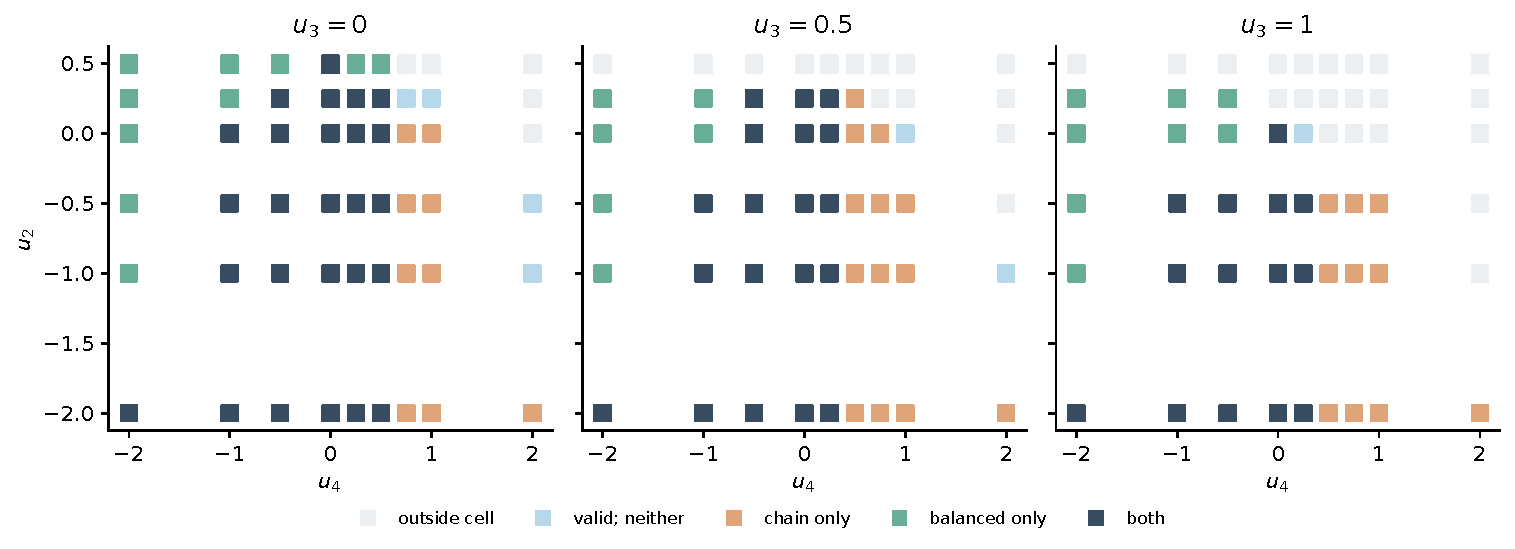
\includegraphics[width=\linewidth]{exact_grid.pdf}
\caption{Exact rational audit, showing the nonnegative $u_3$ slices of the declared grid. Every classification uses rational arithmetic and exact real-root counts. The negative slices have symmetric classifications. The two sparse systems each certify valid data missed by the other.}\label{fig:grid}
\end{figure}

\subsection{Semidefinite closure versus a scalar reference}
For each $d=3,\ldots,8$, we solve 24 boundary problems: 12 equally spaced $u_3$ values in $[-3,3]$ with other tail coordinates zero, followed by 12 tails sampled uniformly from $[-0.6,0.6]^{d-2}$. The seed is 1720406. The scalar implementation enumerates the real stationary roots of the coercive univariate polynomial and evaluates its minimum; its roots are computed in floating point. The SDP independently enforces \eqref{eq:anti} through CVXPY \cite{cvxpy} and Clarabel \cite{clarabel}.

All 144 comparisons finish with solver status \texttt{optimal}. The maximum absolute boundary discrepancy is $5.15\times10^{-9}$, maximum coefficient residual $2.23\times10^{-10}$, and smallest returned matrix eigenvalue $-3.91\times10^{-9}$. These small negative eigenvalues are numerical residuals, not exact PSD certificates. The checks use acceptance thresholds $2\times10^{-6}$ on boundary error and $2\times10^{-7}$ on coefficient/eigenvalue residuals. They corroborate the exact closure proposition on a finite set; they do not certify arbitrary floating-point outputs.

The recorded environment is Python 3.9.6, NumPy 2.0.2, SciPy 1.13.1, SymPy 1.14.0, CVXPY 1.7.5, and Clarabel 0.11.1 on macOS arm64. Solver absolute-gap, relative-gap, and feasibility tolerances are $10^{-9}$, with 300 iterations allowed. Root computations accept stationary roots with imaginary magnitude below $10^{-7}$; no such tolerance enters the rational audit.

\subsection{Near-face sampling and a calibration interpretation}
For $d\in\{4,6,8\}$ and $\delta\in\{0.1,0.03,0.01,0.003,0.001\}$, we generate 2,000 points uniformly in $K_{\delta,1/4}$, using seed 6141720. Uniform sampling in the $\ell_1$ ball uses normalized independent exponential variables, random signs, and the radial factor $U^{1/n}$. The balanced matrix is checked independently for every point. All 30,000 pass. The chain certifies 16,034 overall; selected near-face counts are shown in \cref{tab:near}. These empirical counts illustrate the theorem on its own prescribed geometry, not an application distribution. Increasing dimension need not monotonically decrease finite-$\delta$ rates under this sampling, since the $\ell_1$ ball itself changes shape.

\begin{table}[t]
\centering
\begin{tabular}{rrrrr}
\toprule
$d$ & $\delta$ & Inputs & Chain certified & Balanced certified\\\midrule
4&0.01&2,000&1,044&2,000\\
4&0.001&2,000&316&2,000\\
6&0.01&2,000&870&2,000\\
6&0.001&2,000&25&2,000\\
8&0.01&2,000&1,265&2,000\\
8&0.001&2,000&3&2,000\\\bottomrule
\end{tabular}
\caption{Selected full-dimensional normal-slice samples from the 30,000-point near-face audit. The balanced guarantee applies to all points of each prism, independently of sampling.}\label{tab:near}
\end{table}

A concrete interpretation is a four-channel consistency layer with latent scalar state $t$ and ideal output $(t,t^2,t^3,t^4)$. Given a proposed state $t=0$, one wants to certify that it is globally nearest to the measured output. Consider the synthetic normal perturbations
\[
 u=(0,1/2-\delta,0,z),\quad
 \delta\in\{0.001,0.01,0.05,0.1,0.25\},\quad
 z\in\{-4,-3.9,\ldots,0\}.
\]
The distance difference is $t^2[2\delta+(1-2z)t^2+t^4+t^6]$, so zero is the unique nearest state for all 205 inputs. The balanced system certifies all 205; the chain certifies 20. The result concerns certificate availability. Both formulations encode the same sensor model and the same optimum; a certificate failure does not imply a wrong state estimate.

\begin{figure}[t]
\centering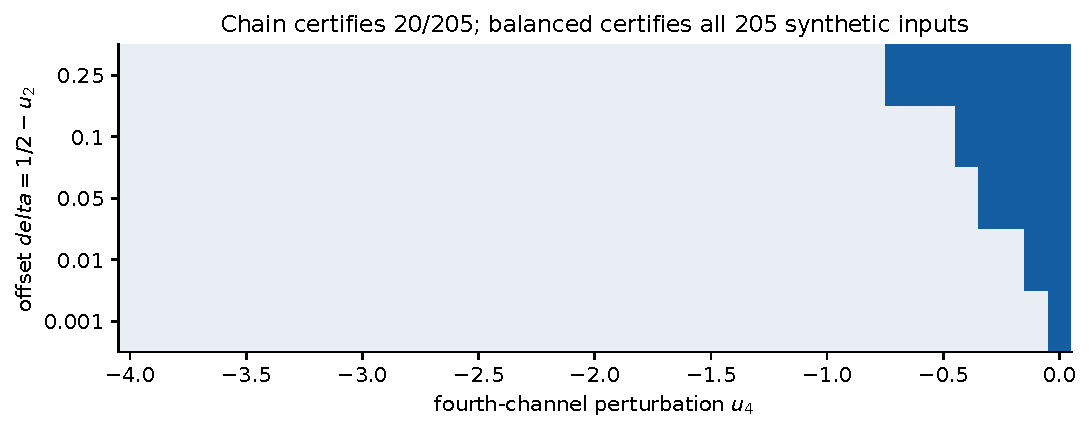
\includegraphics[width=.83\linewidth]{synthetic_calibration.pdf}
\caption{Synthetic four-channel consistency example. Dark cells indicate a chain certificate. Every cell has the same known nearest state and a balanced certificate. Inputs are deliberately selected normal perturbations; the study is not a measured sensor benchmark.}\label{fig:application}
\end{figure}

\section{Implications, scope, and further questions}\label{sec:discussion}
The analysis suggests a diagnostic for a polynomial-model compiler. At a proposed projection, construct the centered Lagrangian matrix and inspect any coordinate whose diagonal approaches zero. A multiplication involving that coordinate creates an off-diagonal coefficient that PSD must suppress. For the family here, this diagnostic exactly predicts the lost face dimensions. A compiler can retain alternative factorizations, add selected quadratic collisions, or fall back to full closure. Because sparse formulations are incomparable, the appropriate decision depends on the anticipated normal directions rather than a universal preference for balanced products.

Potential applications include certifying consistency of polynomial feature vectors, scalar calibration with correlated feature channels after appropriate metric modeling, and preprocessing polynomial optimization models. The present evidence establishes mathematical behavior and a reproducible software diagnostic. It does not establish market demand, patented novelty, improved latency in a production solver, or superiority on multivariate industrial models. The one-dimensional latent variable is also a limitation: direct univariate optimization is often preferable to an SDP for this exact family. Its value here is an analytically controlled test bed for formulation behavior that is harder to isolate in larger systems.

The dimension theorem is local to the distinguished origin and recursive monomial presentations, with an extension to positive diagonal metrics. General positive-definite metrics preserve the availability of full-closure certificates, but the sparse face classification need not have the same form. General polynomial curves may have gaps in their monomial support and need not inherit the same first-order exactness after quadratic closure. Our arguments do not extend that conclusion to arbitrary algebraic varieties.

Several questions remain. Can a small subset of collision quadrics recover a prescribed collection of normal directions without the full quadratic relation space? Can factor choices be optimized from a metric and a specified normal uncertainty set, while controlling sparsity? What replaces the zero-row dimension count when several tangent directions degenerate simultaneously? These questions separate geometric certificate design from increasing relaxation order, and can be tested against the exact family and counterexamples supplied here.

\section*{Data and code availability}
The public repository contains the mathematical implementation, exact verification script, deterministic experiments, raw results, four vector figures, and this \LaTeX\ source. Commands in the repository regenerate the tables and figures. The accompanying software and data release is version 1.0.0, available at \url{https://github.com/shi1720/multiplication-presentations/releases/tag/v1.0.0}. No commercial solver or external dataset is required. The manuscript and its claims should be evaluated together with the stated contribution boundary and counterexamples.

\section*{Funding}
This research did not receive any specific grant from funding agencies in the public, commercial, or not-for-profit sectors.

\section*{Declaration of competing interests}
Shivam Gupta is the founder and CEO of Siloed, a software and AI consultancy. The manuscript discusses potential applications of polynomial-model diagnostics; the research was conducted independently and the code is openly available.

\section*{Author contributions}
Shivam Gupta is the sole author and corresponding author. He reviewed and approved the manuscript and assumes responsibility for its content.

\section*{Declaration of generative AI and AI-assisted technologies in the manuscript preparation process}
OpenAI Codex assisted with literature searches, mathematical development, drafting, and computational experiments; the author reviewed the work and assumes responsibility for its content.

\begin{thebibliography}{99}\small
\bibitem{chs} D. Cifuentes, C. Harris, and B. Sturmfels. The geometry of SDP-exactness in quadratic optimization. \emph{Mathematical Programming} 182 (2020), 399--428. \href{https://doi.org/10.1007/s10107-019-01399-8}{doi:10.1007/s10107-019-01399-8}.
\bibitem{lr} J. Lindberg and J. I. Rodriguez. Invariants of SDP exactness in quadratic programming. \emph{Journal of Symbolic Computation} 122 (2024), 102258. \href{https://doi.org/10.1016/j.jsc.2023.102258}{doi:10.1016/j.jsc.2023.102258}.
\bibitem{eddegree} J. Draisma, E. Horobe\c{t}, G. Ottaviani, B. Sturmfels, and R. R. Thomas. The Euclidean distance degree of an algebraic variety. \emph{Foundations of Computational Mathematics} 16 (2016), 99--149. \href{https://doi.org/10.1007/s10208-014-9240-x}{doi:10.1007/s10208-014-9240-x}.
\bibitem{voronoi} D. Cifuentes, K. Ranestad, B. Sturmfels, and M. Weinstein. Voronoi cells of varieties. \emph{Journal of Symbolic Computation} 109 (2022), 351--366. \href{https://doi.org/10.1016/j.jsc.2020.07.009}{doi:10.1016/j.jsc.2020.07.009}.
\bibitem{mk} M. Mevissen and M. Kojima. SDP relaxations for quadratic optimization problems derived from polynomial optimization problems. \emph{Asia-Pacific Journal of Operational Research} 27 (2010), 15--38. \href{https://doi.org/10.1142/S0217595910002533}{doi:10.1142/S0217595910002533}.
\bibitem{kac} T. Karia, C. S. Adjiman, and B. Chachuat. Assessment of a two-step approach for global optimization of mixed-integer polynomial programs using quadratic reformulation. \emph{Computers \& Chemical Engineering} 165 (2022), 107909. \href{https://doi.org/10.1016/j.compchemeng.2022.107909}{doi:10.1016/j.compchemeng.2022.107909}.
\bibitem{bsv} G. Blekherman, G. G. Smith, and M. Velasco. Sums of squares and varieties of minimal degree. \emph{Journal of the American Mathematical Society} 29 (2016), 893--913. \href{https://doi.org/10.1090/jams/847}{doi:10.1090/jams/847}.
\bibitem{henrion} D. Henrion. Geometry of exactness of moment-SOS relaxations for polynomial optimization. \emph{Optimization Letters} 19 (2025), 1239--1248. \href{https://doi.org/10.1007/s11590-025-02202-8}{doi:10.1007/s11590-025-02202-8}.
\bibitem{cvxpy} S. Diamond and S. Boyd. CVXPY: A Python-embedded modeling language for convex optimization. \emph{Journal of Machine Learning Research} 17(83) (2016), 1--5. \url{https://jmlr.org/papers/v17/15-408.html}.
\bibitem{clarabel} P. J. Goulart and Y. Chen. Clarabel: An interior-point solver for conic programs with quadratic objectives. \emph{Mathematical Programming Computation} (2026). \href{https://doi.org/10.1007/s12532-026-00320-7}{doi:10.1007/s12532-026-00320-7}.
\end{thebibliography}
\end{document}
